% Options for packages loaded elsewhere
% Options for packages loaded elsewhere
\PassOptionsToPackage{unicode}{hyperref}
\PassOptionsToPackage{hyphens}{url}
\PassOptionsToPackage{dvipsnames,svgnames,x11names}{xcolor}
%
\documentclass[
  sn-nature,
]{sn-jnl}


\usepackage{xcolor}
\usepackage{amsmath,amssymb}
\setcounter{secnumdepth}{-\maxdimen} % remove section numbering
\usepackage{iftex}
\ifPDFTeX
  \usepackage[T1]{fontenc}
  \usepackage[utf8]{inputenc}
  \usepackage{textcomp} % provide euro and other symbols
\else % if luatex or xetex
  \usepackage{unicode-math} % this also loads fontspec
  \defaultfontfeatures{Scale=MatchLowercase}
  \defaultfontfeatures[\rmfamily]{Ligatures=TeX,Scale=1}
\fi
\usepackage{lmodern}
\ifPDFTeX\else
  % xetex/luatex font selection
\fi
% Use upquote if available, for straight quotes in verbatim environments
\IfFileExists{upquote.sty}{\usepackage{upquote}}{}
\IfFileExists{microtype.sty}{% use microtype if available
  \usepackage[]{microtype}
  \UseMicrotypeSet[protrusion]{basicmath} % disable protrusion for tt fonts
}{}
\makeatletter
\@ifundefined{KOMAClassName}{% if non-KOMA class
  \IfFileExists{parskip.sty}{%
    \usepackage{parskip}
  }{% else
    \setlength{\parindent}{0pt}
    \setlength{\parskip}{6pt plus 2pt minus 1pt}}
}{% if KOMA class
  \KOMAoptions{parskip=half}}
\makeatother
% Make \paragraph and \subparagraph free-standing
\makeatletter
\ifx\paragraph\undefined\else
  \let\oldparagraph\paragraph
  \renewcommand{\paragraph}{
    \@ifstar
      \xxxParagraphStar
      \xxxParagraphNoStar
  }
  \newcommand{\xxxParagraphStar}[1]{\oldparagraph*{#1}\mbox{}}
  \newcommand{\xxxParagraphNoStar}[1]{\oldparagraph{#1}\mbox{}}
\fi
\ifx\subparagraph\undefined\else
  \let\oldsubparagraph\subparagraph
  \renewcommand{\subparagraph}{
    \@ifstar
      \xxxSubParagraphStar
      \xxxSubParagraphNoStar
  }
  \newcommand{\xxxSubParagraphStar}[1]{\oldsubparagraph*{#1}\mbox{}}
  \newcommand{\xxxSubParagraphNoStar}[1]{\oldsubparagraph{#1}\mbox{}}
\fi
\makeatother


\usepackage{longtable,booktabs,array}
\usepackage{calc} % for calculating minipage widths
% Correct order of tables after \paragraph or \subparagraph
\usepackage{etoolbox}
\makeatletter
\patchcmd\longtable{\par}{\if@noskipsec\mbox{}\fi\par}{}{}
\makeatother
% Allow footnotes in longtable head/foot
\IfFileExists{footnotehyper.sty}{\usepackage{footnotehyper}}{\usepackage{footnote}}
\makesavenoteenv{longtable}
\usepackage{graphicx}
\makeatletter
\newsavebox\pandoc@box
\newcommand*\pandocbounded[1]{% scales image to fit in text height/width
  \sbox\pandoc@box{#1}%
  \Gscale@div\@tempa{\textheight}{\dimexpr\ht\pandoc@box+\dp\pandoc@box\relax}%
  \Gscale@div\@tempb{\linewidth}{\wd\pandoc@box}%
  \ifdim\@tempb\p@<\@tempa\p@\let\@tempa\@tempb\fi% select the smaller of both
  \ifdim\@tempa\p@<\p@\scalebox{\@tempa}{\usebox\pandoc@box}%
  \else\usebox{\pandoc@box}%
  \fi%
}
% Set default figure placement to htbp
\def\fps@figure{htbp}
\makeatother

\ifLuaTeX
  \usepackage{luacolor}
  \usepackage[soul]{lua-ul}
\else
  \usepackage{soul}
\fi

% definitions for citeproc citations
\NewDocumentCommand\citeproctext{}{}
\NewDocumentCommand\citeproc{mm}{%
  \begingroup\def\citeproctext{#2}\cite{#1}\endgroup}
\makeatletter
 % allow citations to break across lines
 \let\@cite@ofmt\@firstofone
 % avoid brackets around text for \cite:
 \def\@biblabel#1{}
 \def\@cite#1#2{{#1\if@tempswa , #2\fi}}
\makeatother
\newlength{\cslhangindent}
\setlength{\cslhangindent}{1.5em}
\newlength{\csllabelwidth}
\setlength{\csllabelwidth}{3em}
\newenvironment{CSLReferences}[2] % #1 hanging-indent, #2 entry-spacing
 {\begin{list}{}{%
  \setlength{\itemindent}{0pt}
  \setlength{\leftmargin}{0pt}
  \setlength{\parsep}{0pt}
  % turn on hanging indent if param 1 is 1
  \ifodd #1
   \setlength{\leftmargin}{\cslhangindent}
   \setlength{\itemindent}{-1\cslhangindent}
  \fi
  % set entry spacing
  \setlength{\itemsep}{#2\baselineskip}}}
 {\end{list}}
\usepackage{calc}
\newcommand{\CSLBlock}[1]{\hfill\break\parbox[t]{\linewidth}{\strut\ignorespaces#1\strut}}
\newcommand{\CSLLeftMargin}[1]{\parbox[t]{\csllabelwidth}{\strut#1\strut}}
\newcommand{\CSLRightInline}[1]{\parbox[t]{\linewidth - \csllabelwidth}{\strut#1\strut}}
\newcommand{\CSLIndent}[1]{\hspace{\cslhangindent}#1}



\setlength{\emergencystretch}{3em} % prevent overfull lines

\providecommand{\tightlist}{%
  \setlength{\itemsep}{0pt}\setlength{\parskip}{0pt}}





%%%% Standard Packages

\usepackage{graphicx}%
\usepackage{multirow}%
\usepackage{amsmath,amssymb,amsfonts}%
\usepackage{amsthm}%
\usepackage{mathrsfs}%
\usepackage[title]{appendix}%
\usepackage{xcolor}%
\usepackage{textcomp}%
\usepackage{manyfoot}%
\usepackage{booktabs}%
\usepackage{algorithm}%
\usepackage{algorithmicx}%
\usepackage{algpseudocode}%
\usepackage{listings}%
\usepackage{orcidlink}
%%%%

\raggedbottom
\usepackage{fontspec}

% Pick a test font you KNOW exists (verify with: fc-list | grep -i "Arial")
\setmainfont{Helvetica Neue}
\setsansfont{Helvetica Neue}

% Optional: if you want another later, change both above to e.g. Fira Sans.

% Force any \fontfamily{\sfdefault} back to main:
\renewcommand{\sfdefault}{\rmdefault}

% Patch section/figure/etc fonts that embed \fontfamily{\sfdefault}
\makeatletter
\def\sectionfont{\reset@font\fontsize{14bp}{16bp}\bfseries\selectfont}
\def\subsectionfont{\reset@font\fontsize{12bp}{14bp}\bfseries\selectfont}
\def\subsubsectionfont{\reset@font\fontsize{11bp}{13bp}\bfseries\selectfont}
\def\paragraphfont{\reset@font\fontsize{10bp}{12bp}\bfseries\itshape\selectfont}
\def\bmheadfont{\reset@font\fontsize{10bp}{12bp}\bfseries\selectfont}
\def\figurecaptionfont{\reset@font\fontsize{8}{9.5}\selectfont}
\def\quotefont{\reset@font\fontsize{9}{11}\selectfont}
\def\eqnheadfont{\reset@font\fontsize{16}{18}\bfseries\selectfont}
% Bibliography font override
\def\bibfont{\reset@font\normalsize\selectfont}
\makeatother

% Reduce white space: widen text block and adjust margins
\geometry{
  paperwidth=210mm,
  paperheight=297mm,
  top=25.4mm,
  bottom=25.4mm,
  left=31.7mm,
  right=31.7mm,
  headsep=2.54mm,
  footskip=12mm,
  % For single-column pages
  textwidth=174mm,
  textheight=245mm
}
% If you use double-column option, uncomment:
% \if@iicol
%   \geometry{text={174mm,240mm}}
% \fi
\usepackage{lineno}
\linenumbers
\linespread{1.5}
\makeatletter
\@ifpackageloaded{float}{}{\usepackage{float}}
\floatstyle{plain}
\@ifundefined{c@chapter}{\newfloat{suppfig}{h}{losuppfig}}{\newfloat{suppfig}{h}{losuppfig}[chapter]}
\floatname{suppfig}{Supplemental Figure}
\newcommand*\listofsuppfigs{\listof{suppfig}{List of Supplementary Figures}}
\makeatother
\makeatletter
\@ifpackageloaded{caption}{}{\usepackage{caption}}
\AtBeginDocument{%
\ifdefined\contentsname
  \renewcommand*\contentsname{Table of contents}
\else
  \newcommand\contentsname{Table of contents}
\fi
\ifdefined\listfigurename
  \renewcommand*\listfigurename{List of Figures}
\else
  \newcommand\listfigurename{List of Figures}
\fi
\ifdefined\listtablename
  \renewcommand*\listtablename{List of Tables}
\else
  \newcommand\listtablename{List of Tables}
\fi
\ifdefined\figurename
  \renewcommand*\figurename{Figure}
\else
  \newcommand\figurename{Figure}
\fi
\ifdefined\tablename
  \renewcommand*\tablename{Table}
\else
  \newcommand\tablename{Table}
\fi
}
\@ifpackageloaded{float}{}{\usepackage{float}}
\floatstyle{ruled}
\@ifundefined{c@chapter}{\newfloat{codelisting}{h}{lop}}{\newfloat{codelisting}{h}{lop}[chapter]}
\floatname{codelisting}{Listing}
\newcommand*\listoflistings{\listof{codelisting}{List of Listings}}
\makeatother
\makeatletter
\makeatother
\makeatletter
\@ifpackageloaded{caption}{}{\usepackage{caption}}
\@ifpackageloaded{subcaption}{}{\usepackage{subcaption}}
\makeatother
\usepackage{bookmark}
\IfFileExists{xurl.sty}{\usepackage{xurl}}{} % add URL line breaks if available
\urlstyle{same}
\hypersetup{
  pdftitle={Benchmarking sequence and structure homology based methods for eukaryotic virus protein annotation},
  pdfauthor={Lander De Coninck; Uri Neri; Simon Roux},
  colorlinks=true,
  linkcolor={black},
  filecolor={Maroon},
  citecolor={Blue},
  urlcolor={Blue},
  pdfcreator={LaTeX via pandoc}}


\title[Benchmarking sequence and structure homology based methods for
eukaryotic virus protein annotation]{Benchmarking sequence and structure
homology based methods for eukaryotic virus protein annotation}

% author setup
\author*[1]{\fnm{Lander} \sur{De
Coninck}\orcidlink{0000-0001-6847-2379}}\email{lander.deconinck@kuleuven.be}\author[2]{\fnm{Uri} \sur{Neri}\orcidlink{0000-0003-0894-2484}}\email{uneri@lbl.gov}\author[2]{\fnm{Simon} \sur{Roux}\orcidlink{0000-0002-5831-5895}}\email{sroux@lbl.gov}
% affil setup
\affil[1]{\orgname{KU Leuven}%
, \orgdiv{Microbiology, Immunology and Transplantation}%
, \orggroup{Clincial and Epidemiological Virology}%
, \orgaddress{%
  \street{Herestraat 49, box 1040}%
  , \city{Leuven}%
  %
  , \postcode{3000}%
  , \country{Belgium}%
}}
\affil[2]{\orgname{Lawrence Berkeley National Laboratory}%
, \orgdiv{DOE Joint Genome Institute}%
%
, \orgaddress{%
  \street{Cyclotron Road 1}%
  , \city{Berkeley}%
  %
  , \postcode{CA 94720}%
  , \country{USA}%
}}

% abstract 


% keywords

\begin{document}
\maketitle


\section{Abstract}\label{abstract}

\section{Introduction}\label{introduction}

\section{Results \& Discussion}\label{results-discussion}

\subsection{Dataset overview}\label{dataset-overview}

\begin{itemize}
\tightlist
\item
  general overview of data and structures

  \begin{itemize}
  \tightlist
  \item
    TODO: kingdom distribution (proteins vs species)
  \end{itemize}
\item
  performance of methods in hits
\item
  comparison of methods in shared hits
\item
  comparison of functional annotation per method to original
\item
  how many are informative annotations

  \begin{itemize}
  \tightlist
  \item
    TODO: which conversions from hypothetical protein to informative
    (phages?)
  \end{itemize}
\item
  computational benchmark (roughly)
\end{itemize}

\begin{figure}

\centering{

\pandocbounded{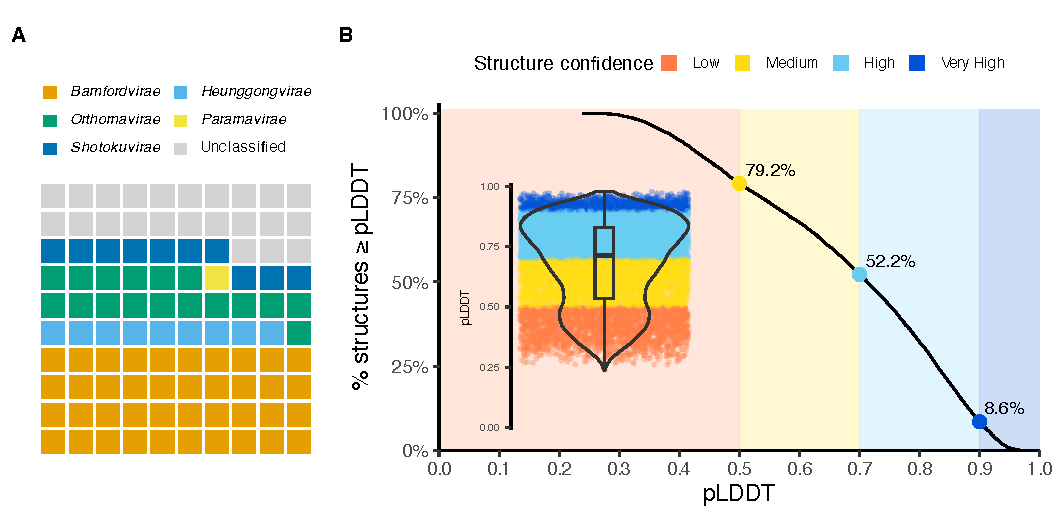
\includegraphics[keepaspectratio]{../figures/dataset_overview.pdf}}

}

\caption{\label{fig-overview}A) Waffle plot showing the distribution of
the number of proteins from the different viral Kingdoms. Each tile
roughly corresponds to 110 proteins. B) A cumulative distribution
function plot showing the percentage of predicted structures from the
test set with a pLDDT score above the pLDDT score on the x-axis. The
inset shows a violin- and boxplot with all pLDDT scores from the
predicted structures (n=11,467).}

\end{figure}%

Figure~\ref{fig-overview}

\begin{figure}

\centering{

\pandocbounded{
\includegraphics[keepaspectratio]{../figures/hits_per_method.pdf}}

}

\caption{\label{fig-hits}Bar plot showing the number of proteins that
got a hit against the BFVD shown per method before and after filtering
the reported results on e-value lower than 1e-3.}

\end{figure}%

Figure~\ref{fig-hits}

\section{Conclusion}\label{conclusion}

\section{Material and Methods}\label{material-and-methods}

\subsection{Dataset selection}\label{dataset-selection}

\subsubsection{Test set}\label{test-set}

To benchmark different methods for eukaryotic virus protein annotation,
we selected 10\% of the exemplar species in ICTV's Virus Metadata
Resource (VMR) v40.2 that did not have bacteria or archaea as designated
host (n=1,000). We subsequently extracted their GenBank accession
numbers (n=1,402) and downloaded all associated proteins (n=11,360).

Protein sequences that were longer than 2,500 amino acids were split
into multiple chunks of maximum 2,500 amino acids so that structure
prediction with Boltz-2\textsuperscript{1} would not run out of GPU
memory (see \hyperref[computational-benchmarking]{below}). This resulted
in a final test set of 11,467 protein sequences from 1,000 eukaryotic
virus species.

\subsubsection{Database}\label{database}

The BFVD\textsuperscript{2} was used as the reference database for both
sequence and structure homology-based annotation. The BFVD is a
comprehensive database of predicted protein structures from the viral
sequence representatives of the UniRef30 clusters. UniRef30 is a UniProt
database that clusters protein sequences at 30\% sequence identity and
selects a representative sequence for each cluster, these
representatives thus have a UniProt accession. Since a substantial
amount of BFVD's included proteins are no longer available in UniProtKB
as they are not part of reference proteomes, we converted their UniProt
accessions to UniParc IDs.

Functional categories for each BFVD entry were derived from protein
names associated with the corresponding UniParc IDs (could be from
UniProtKB/TrEMBL, RefSeq and/or GenBank) for eukaryotic viruses (also
see \hyperref[functional-classifier]{below}) or by classifying them into
PHROG-like\textsuperscript{3} categories with Empathi\textsuperscript{4}
in the case of bacteriophage proteins. The distinction between
eukaryotic virus and bacteriophage proteins was made based on the taxid
information from the UniParc protein ID.

The BFVD database was further converted into the required formats the
search tools used in this benchmarking effort (see
\hyperref[sequence-homology-based-annotation]{sequence} and
\hyperref[structure-homology-based-annotation]{structure} homology-based
annotation).

\subsection{Functional classifier}\label{functional-classifier}

Functional categories for eukaryotic virus proteins were designed with
Perplexity AI in deep research mode using the following prompt: ``Can
you give me an exhaustive list of common protein functions in eukaryotic
viruses? Use https://viralzone.expasy.org and
https://ictv.global/report/genome as sources. Give me a machine readable
file with all these functional categories.'' The resulting functional
categories were further manually curated to ensure that they were
mutually exclusive. The final list of functional categories is available
in \hl{Supplementary Table 1}.

A custom script generated by Perplexity AI was used to assign functional
categories to BFVD proteins based on all their protein names from
UniParc in a JSON file. The script uses pattern matching to assign the
most appropriate functional category to each protein. If no keywords
match, the protein is assigned to the ``Hypothetical Protein'' category.
The prompt to generate the classifier script was: ``Write me a script
that classifies the proteins in the uploaded JSON file (as specific as
possible) into these functional categories, also if there are proteins
in this file that do not fit in one of your proposed categories search
new sources and create new functional categories.''. Followed up by:
``Split the polymerase category in RNA-dependent RNA polymerase, DNA
polymerase and reverse transcriptase. In addition split the
Capsid/Nucleocapsid/Core Structural into Capsid and Nucleocapsid
categories. Split helicase and NTPase.''.

The pattern matching rules, functional categories, and classification
script were subsequently refined through manual curation to optimize the
functional assignment based on protein names.

The same functional classifier script was also used on the protein names
from our test set to assign functional categories to the eukaryotic
virus proteins downloaded from the ICTV exemplar species.

\subsection{Sequence homology-based
annotation}\label{sequence-homology-based-annotation}

For sequence homology annotation, we used three state-of-the-art tools
widely used in functional annotation pipelines and sequence similarity
searches. As gold standard, blastp\textsuperscript{5} was used with an
e-value cutoff of 1e-3. In addition, we used diamond\textsuperscript{6}
in sensitive mode and mmseqs2\textsuperscript{7} with default settings;
both have a default e-value cutoff of 1e-3.

\subsection{Structure prediction}\label{structure-prediction}

For the structure prediction of our test set proteins, we relied on
Boltz-2\textsuperscript{1} (default settings) with multiple sequence
alignments (MSAs) generated by a local, adapted ColabFold
installation\textsuperscript{8} (see
\url{https://github.com/gbouras13/colabfoldv}). To increase the depth
and diversity of the MSAs, we used the default ColabFold sequence
databases, supplemented with extra \emph{Orthornavirae}
sequences\textsuperscript{9} and viral sequences used in the structure
prediction for the Phold database\textsuperscript{10}. Structures were
predicted on an NVIDIA H100 GPU with 80GB of VRAM.

\subsection{Structure homology-based
annotation}\label{structure-homology-based-annotation}

\subsubsection{ProstT5}\label{prostt5}

\subsubsection{TEA}\label{tea}

\subsubsection{Foldseek}\label{foldseek}

\subsubsection{Reseek}\label{reseek}

\subsection{Computational
benchmarking}\label{computational-benchmarking}

\begin{itemize}
\tightlist
\item
  hyperfine
\end{itemize}

\phantomsection\label{refs}
\begin{CSLReferences}{0}{0}
\bibitem[\citeproctext]{ref-passaroBoltz2AccurateEfficient2025}
\CSLLeftMargin{1. }%
\CSLRightInline{Passaro, S. \emph{et al.} Boltz-2: {Towards Accurate}
and {Efficient Binding Affinity Prediction}. 2025.06.14.659707 (2025)
doi:\href{https://doi.org/10.1101/2025.06.14.659707}{10.1101/2025.06.14.659707}.}

\bibitem[\citeproctext]{ref-kimBFVDLargeRepository2025}
\CSLLeftMargin{2. }%
\CSLRightInline{Kim, R. S., Levy Karin, E., Mirdita, M., Chikhi, R. \&
Steinegger, M. \href{https://doi.org/10.1093/nar/gkae1119}{{BFVD}---a
large repository of predicted viral protein structures}. \emph{Nucleic
Acids Research} \textbf{53}, D340--D347 (2025).}

\bibitem[\citeproctext]{ref-terzianPHROGFamiliesProkaryotic2021}
\CSLLeftMargin{3. }%
\CSLRightInline{Terzian, P. \emph{et al.}
\href{https://doi.org/10.1093/nargab/lqab067}{{PHROG}: Families of
prokaryotic virus proteins clustered using remote homology}. \emph{NAR
Genomics and Bioinformatics} \textbf{3}, lqab067 (2021).}

\bibitem[\citeproctext]{ref-boulayEmpathiEmbeddingbasedPhage2025}
\CSLLeftMargin{4. }%
\CSLRightInline{Boulay, A., Leprince, A., Enault, F., Rousseau, E. \&
Galiez, C. \href{https://doi.org/10.1038/s41467-025-64177-5}{Empathi:
Embedding-based phage protein annotation tool by hierarchical
assignment}. \emph{Nature Communications} \textbf{16}, 9114 (2025).}

\bibitem[\citeproctext]{ref-altschulBasicLocalAlignment1990}
\CSLLeftMargin{5. }%
\CSLRightInline{Altschul, S. F., Gish, W., Miller, W., Myers, E. W. \&
Lipman, D. J. \href{https://doi.org/10.1016/S0022-2836(05)80360-2}{Basic
local alignment search tool}. \textbf{215}, 403--410 (1990).}

\bibitem[\citeproctext]{ref-buchfinkSensitiveProteinAlignments2021}
\CSLLeftMargin{6. }%
\CSLRightInline{Buchfink, B., Reuter, K. \& Drost, H.-G.
\href{https://doi.org/10.1038/s41592-021-01101-x}{Sensitive protein
alignments at tree-of-life scale using {DIAMOND}}. \emph{Nature Methods}
\textbf{18}, 366--368 (2021).}

\bibitem[\citeproctext]{ref-steineggerMMseqs2EnablesSensitive2017}
\CSLLeftMargin{7. }%
\CSLRightInline{Steinegger, M. \& Söding, J.
\href{https://doi.org/10.1038/nbt.3988}{{MMseqs2} enables sensitive
protein sequence searching for the analysis of massive data sets}.
\emph{Nature Biotechnology} \textbf{35}, 1026--1028 (2017).}

\bibitem[\citeproctext]{ref-mirditaColabFoldMakingProtein2022}
\CSLLeftMargin{8. }%
\CSLRightInline{Mirdita, M. \emph{et al.}
\href{https://doi.org/10.1038/s41592-022-01488-1}{{ColabFold}: Making
protein folding accessible to all}. \emph{Nature Methods} \textbf{19},
679--682 (2022).}

\bibitem[\citeproctext]{ref-mutzProteinStructuromeOrthornavirae2024}
\CSLLeftMargin{9. }%
\CSLRightInline{Mutz, P. \emph{et al.}
\href{https://doi.org/10.1128/mbio.03200-24}{The protein structurome of
{Orthornavirae} and its dark matter}. \emph{mBio} \textbf{16},
e03200--24 (2024).}

\bibitem[\citeproctext]{ref-bourasProteinStructureinformedBacteriophage2026}
\CSLLeftMargin{10. }%
\CSLRightInline{Bouras, G. \emph{et al.}
\href{https://doi.org/10.1093/nar/gkaf1448}{Protein structure-informed
bacteriophage genome annotation with {Phold}}. \emph{Nucleic Acids
Research} \textbf{54}, (2026).}

\end{CSLReferences}




\end{document}
